\section{Objective}\label{sec:objective}

The primary objective of this project is to build a machine that can effectively compete with a human in foosball.
More specifically, the machine should be able to:

\begin{itemize}
    \item Defend against balls traveling at speeds of up to $7m/s$.
    This is approximately the speed achieved by normal players when they try to shoot fast.
    \item Shoot the ball back with a speed of $7m/s$.
    \item Achieve a positional precision of $0.1mm$, which is circa the accuracy of normal stepper motors (including the mechanics to move the players).
\end{itemize}


\section{Motors}\label{sec:motors}

\subsection{Objectives}\label{subsec:objectives}
We want to be able to defend a ball with a velocity of maximum $v=7m/s$.

\subsection{Table measurements}\label{subsec:table_measurements}
This picture shows the table with the measurements:

\begin{tikzpicture}
    \node[anchor=south west,inner sep=0] (image) at (0,0) {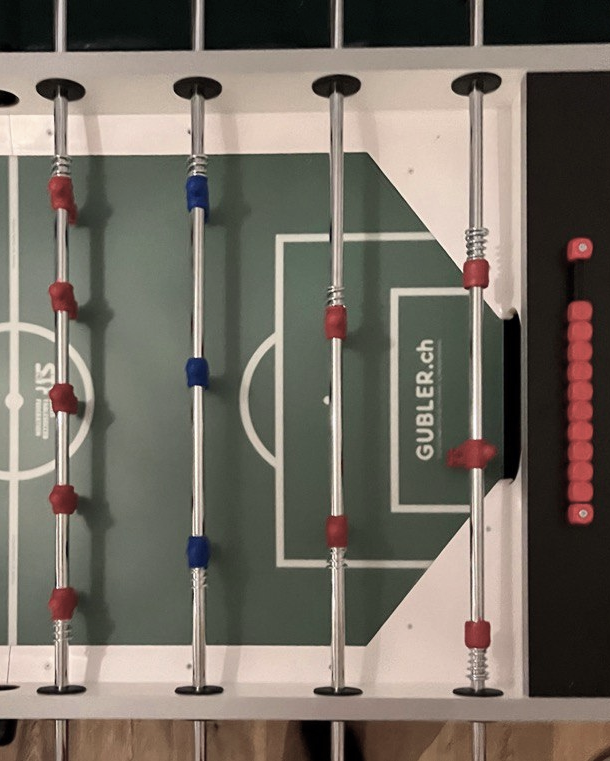
\includegraphics[width=0.5\textwidth]{../photos/foosball_table}};
    \begin{scope}
        [x={(image.south east)},y={(image.north west)}]
%        \draw[help lines,xstep=.1,ystep=.1] (0,0) grid (1,1);
%        \foreach \x in {0,1,...,9} { \node [anchor=north] at (\x/10,0) {0.\x}; }
%        \foreach \y in {0,1,...,9} { \node [anchor=east] at (0,\y/10) {0.\y}; }
        \def \tubex {0.76};
%        \draw[red,ultra thick,rounded corners] (0.62,0.65) rectangle (0.78,0.75);
        \draw[<->,blue!80!black!50,rounded corners, line width=1.5mm] (\tubex, 0.9)  -- (\tubex, 0.65) node[below, left] {\huge \textbf{180mm}};
        \draw[<->,blue!80!black!100,rounded corners, line width=1.5mm] (0.85, 0.9)  -- (0.85, 0.09) node[pos=0.85, left] {\huge \textbf{700mm}};

    \end{scope}
\end{tikzpicture}

\todo{The calculations dont make completly sense, i think i made a mistake somewhere and bought an overpowered motor, which is fine i guess}
\subsection{Calculations for the moving motor}\label{subsec:moving_motor}
The distance from the attacker to the goal is $s=0.4m$.
That means we have stop the ball in time t, where
\begin{equation}
    \label{eq:stopping_time}
    t = \frac{s}{v} = \frac{0.4m}{7m/s} = 0.057s.
\end{equation}
Which is not a lot of time to process the image and move the motors.
The goalkeeper has to travel a maximum distance of 0.2m in 0.057s, that means we have an average velocity of
\begin{equation}
    \label{eq:average_velocity}
    v = \frac{s}{t} = \frac{0.2m}{0.057s} = 3.5m/s
\end{equation}
Which means we need a top speed of at least $2\cdot3.5m/s=7m/s$, as the motors have to accelerate and decelerate.
We also need to be able to move the motors in 0.057s, which means we need a maximum acceleration $a$ of
\begin{equation}
    \label{eq:acceleration}
    a = \frac{v}{t} = \frac{7m/s}{0.057s} = 122.8m/s^2.
\end{equation}
We assume that the weight of the tubes is $m \approx 0.1kg$.
The torque needed to move the tubes is
\begin{equation}
    \label{eq:torque}
    \tau = F \cdot r = m \cdot a \cdot r = 0.1kg \cdot 122.8m/s^2 \cdot 0.083m \approx 1Nm
\end{equation}
assuming the radius of the gear is 8.3cm.
And the required top rational speed (measured in rotations per minute $\text{RPM}$) is
\begin{equation}
    \label{eq:top_rpm}
    \frac{v}{2\pi r} \cdot 60 = \frac{7m/s}{2\pi \cdot 0.083m} \cdot 60 \approx 800\text{RPM}.
\end{equation}
A Motor that fits those requirements is the \textbf{PD42-3-1141} from \textbf{Trinamic}.

\subsection{Calculations for the rotating motor}\label{subsec:rotating_motor}
The ball has a mass $m=17g$.
We assume that we have an angle of $45\deg$ ($=\frac{\pi}{4}$ in radians) to accelerate the ball.
\\
\begin{center}

    \tikzset{
        testpic/.pic={
            \node at (0.05,-0.35) {
\includegraphics[height=3.2cm] {../photos/foosball_player}};
        },
        testpic2/.pic={
            \node at (0.05,-0.35) {
\includegraphics[height=3.2cm] {../photos/foosball_player}};
        },
    }

    \begin{tikzpicture}
        \def \r {2cm}
        \def \rsmall {0.5}
        \def \angle {45}
        \pic[rotate=45/2,transform shape] at (0,0) {testpic};
        \pic[rotate=-45/2,transform shape] at (0,0) {testpic2};
        \draw (0,0) -- ({-sin(\angle / 2)*\r}, {-cos(\angle / 2)*\r});
        \draw (0,0) -- ({sin(\angle / 2)*\r}, {-cos(\angle / 2)*\r}) node[right, midway] {$r=70\text{mm}$};
        \draw ({-sin(\angle / 2)*\rsmall}, {-cos(\angle / 2)*\rsmall}) arc(270-\angle/2:270+\angle/2:\rsmall) node[midway,below] {$45\deg$};
        \draw[->] ({-sin(\angle / 2)*\r}, {-cos(\angle / 2)*\r}) arc(270-\angle/2:270+\angle/2:\r) node[midway,below] {$l$};
%        \draw () circle (\r);
    \end{tikzpicture}
\end{center}
%    \\
That means we have the distance $a$ to accelerate the ball.
\begin{equation}
    \label{eq:distance}
    l = r \cdot \frac{\pi}{4} = 70mm \cdot \frac{\pi}{4} = 55mm
\end{equation}
The goal is to shoot the ball back at a speed of 7m/s.
The time to accelerate the ball is
\begin{equation}
    \label{eq:time}
    t = \frac{2\pi\cdot r}{v} = \frac{2\pi\cdot 70mm}{7m/s} = \frac{\pi}{50} \approx 0.06s
\end{equation}
The maximum speed can easily be calculated with
\begin{equation}
    \label{eq:max_speed}
    \omega = \frac{60s/min}{t} = \frac{60s/min}{0.6s/rotation} = 1000\text{RPM}
\end{equation}
\todo{Compute the torque needed to accelerate the ball}
For the motor that just rotates the figure we can use a DC motor with gears and an encoder.
% Pololu 10:1 Metal Gearmotor 37Dx65L mm 12V with 64 CPR Encoder (Helical Pinion) 4758
A motor that fits those requirements is the \textbf{Pololu 10:1 Metal Gearmotor 37Dx65L mm 12V with 64 CPR Encoder (Helical Pinion) 4758}.


\section{Camera}\label{sec:camera}

\subsection{Optics}\label{subsec:lens}
To achieve our goal of defending against balls at speed of up to $7m/s$, we need a camera that can capture the entire table at a framerate of at least 200fps.
A sensor that achieves this is the \textbf{IMX287 CMOS} sensor from \textbf{Sony}.
This sensor has a width of $4.98\text{mm}$.
Here is a schematic of the approximate setup for the camera:\\
\begin{center}\begin{tikzpicture}
    \draw (0,0) -- (0, 5);
    \draw (0, 5) -- (10, 5);
    \draw (10, 5) -- (10, 0);

    \draw (1,0) -- (1, 4);
    \draw (1, 4) -- (9, 4);
    \draw (9, 4) -- (9, 0);

    \draw (4.5, 0) -- (5.5, 0) node[below] {Sensor (4.98mm)};

    \pgfmathsetmacro{\lensRadius}{1}
    \pgfmathsetmacro{\lensHeight}{0.5}
    \pgfmathsetmacro{\startAngle}{asin(\lensHeight/\lensRadius)}

    \draw [fill=blue!15]  (4.5,\lensHeight)
    arc[start angle=180-\startAngle+90,delta angle=2*\startAngle,radius=\lensRadius]
    arc[start angle=-\startAngle+90,delta angle=2*\startAngle,radius=\lensRadius]
    -- cycle; % to get a better line end

    \draw[blue] (1, 4) -- (4.5, \lensHeight);
    \draw[blue] (4.5, \lensHeight) -- (5.5, 0);

    \draw[blue] (9, 4) -- (5.5, \lensHeight);
    \draw[blue] (5.5, \lensHeight) -- (4.5, 0);

    \draw[green] (1, 4) -- (5.5, \lensHeight);
    \draw[green] (5.5, \lensHeight) -- (5.5, 0);

    \draw[green] (9, 4) -- (4.5, \lensHeight);
    \draw[green] (4.5, \lensHeight) -- (4.5, 0);

    \draw (6.5, 0.5) node[]{Lens}
    \draw[<->] (5, 0.70) -- (5, 4) node[midway, right] {d};
    \draw[<->] (1, 4.2) -- (9, 4.2) node[above, midway] {FoV};
\end{tikzpicture}\end{center}\\

\paragraph{Lens Equation}\label{par:lens_equation}

The relationship between the object width (FoV), sensor width, and distance to the object is given by:
\begin{equation}
    \text{Object Width (FoV)} = \text{Sensor Width} \times \frac{\text{Distance to Object (d)}}{\text{Focal Length (f)}}\label{eq:lens_equation}
\end{equation}


In our case $d = 700mm$ and our Field of View (FoV) is $1200mm$.
Now we solve for the focal length $f$:
\begin{equation}
    \label{eq:focal_length}
    f = \frac{\text{Sensor Width} \times \text{Distance to Object (d)}}{\text{Object Width (FoV)}} = \frac{4.98\text{mm} \times 700\text{mm}}{1200\text{mm}} = 2.9\text{mm}
\end{equation}
% Arducam 2.8-12mm Varifocal C-Mount Lens for Raspberry Pi HQ Camera, with C-CS Adapter
A lens that satisfies these requirements is the \textbf{Arducam 2.8-12mm Varifocal C-Mount Lens for Raspberry Pi HQ Camera, with C-CS Adapter} with a focal length of $2.8-12mm$.